%FOR PDFLATEX USE ONLY
\documentclass[a4paper,12pt]{article}

\usepackage{amssymb,amsmath} %math symbols

\usepackage[margin=2cm]{geometry} %paper geometry

\usepackage[utf8]{inputenc} %allows unicode (including russian) source file
\usepackage[russian]{babel} %docment in russian-style
\usepackage[utf8]{inputenc}
%\usepackage[unicode]{hyperref} %links inside of the text
\usepackage[pdftex]{graphicx} %includegraphics pictures
\usepackage{cmlgc} %bold text

\usepackage{array} %arrays

%\usepackage{wrapfig}
%\usepackage{array}
%\usepackage{lipsum}
%\usepackage{esvect}
%\usepackage{hyperref}

\usepackage{subfig}
%\usepackage{calc}
%\usepackage{pgfplots,tikz,circuitikz}
%\usepackage{tkz-euclide}

\begin{document}

\begin{center}
  \LARGE{Работа 2.4.1}\\[0.2cm]
  \LARGE{Определение теплоты испарения жидкости}\\[0.2cm]
  \large{Панферов Андрей}\\[0.2cm]
\end{center}  
  

\section{Аннотация}

В данной работе измеряется давление насыщенного пара жидкости при разной температуре, по полученным данным вычисляется теплота её испарения с помощью уравнения Клапейрона–Клаузиуса.

\section{Теоретические сведения}
Испарением называется переход вещества из жидкого в газообразное состояние. Чтобы испарение проходило без изменения температуры, к жидкости нужно подводить тепло. Количество теплоты, необходимое для изо- термического испарения одного моля жидкости при внешнем давлении, равном упругости ее насыщенных паров, называется \textit{молярной теплотой испарения}. \\
В настоящей работе для определения теплоты испарения применен косвенный метод, основанный на формуле Клапейрона--Клаузиуса

\begin{equation*}
\frac{dP}{dT}=\frac{\mu L}{T(V_2-V_1)}
\end{equation*}

С помощью уравнения Ван-дер-Ваальса можно получить зависимость P(T), с помощью которой определить искомую величину. 

\begin{equation*}
(P+\frac{a}{V^2})(V-b)=RT
\end{equation*}

В таблице ниже приведены все значения параметров различных жидкостей уранения Ван-дер-Ваальса в условиях данного опыта. 

\begin{center}

  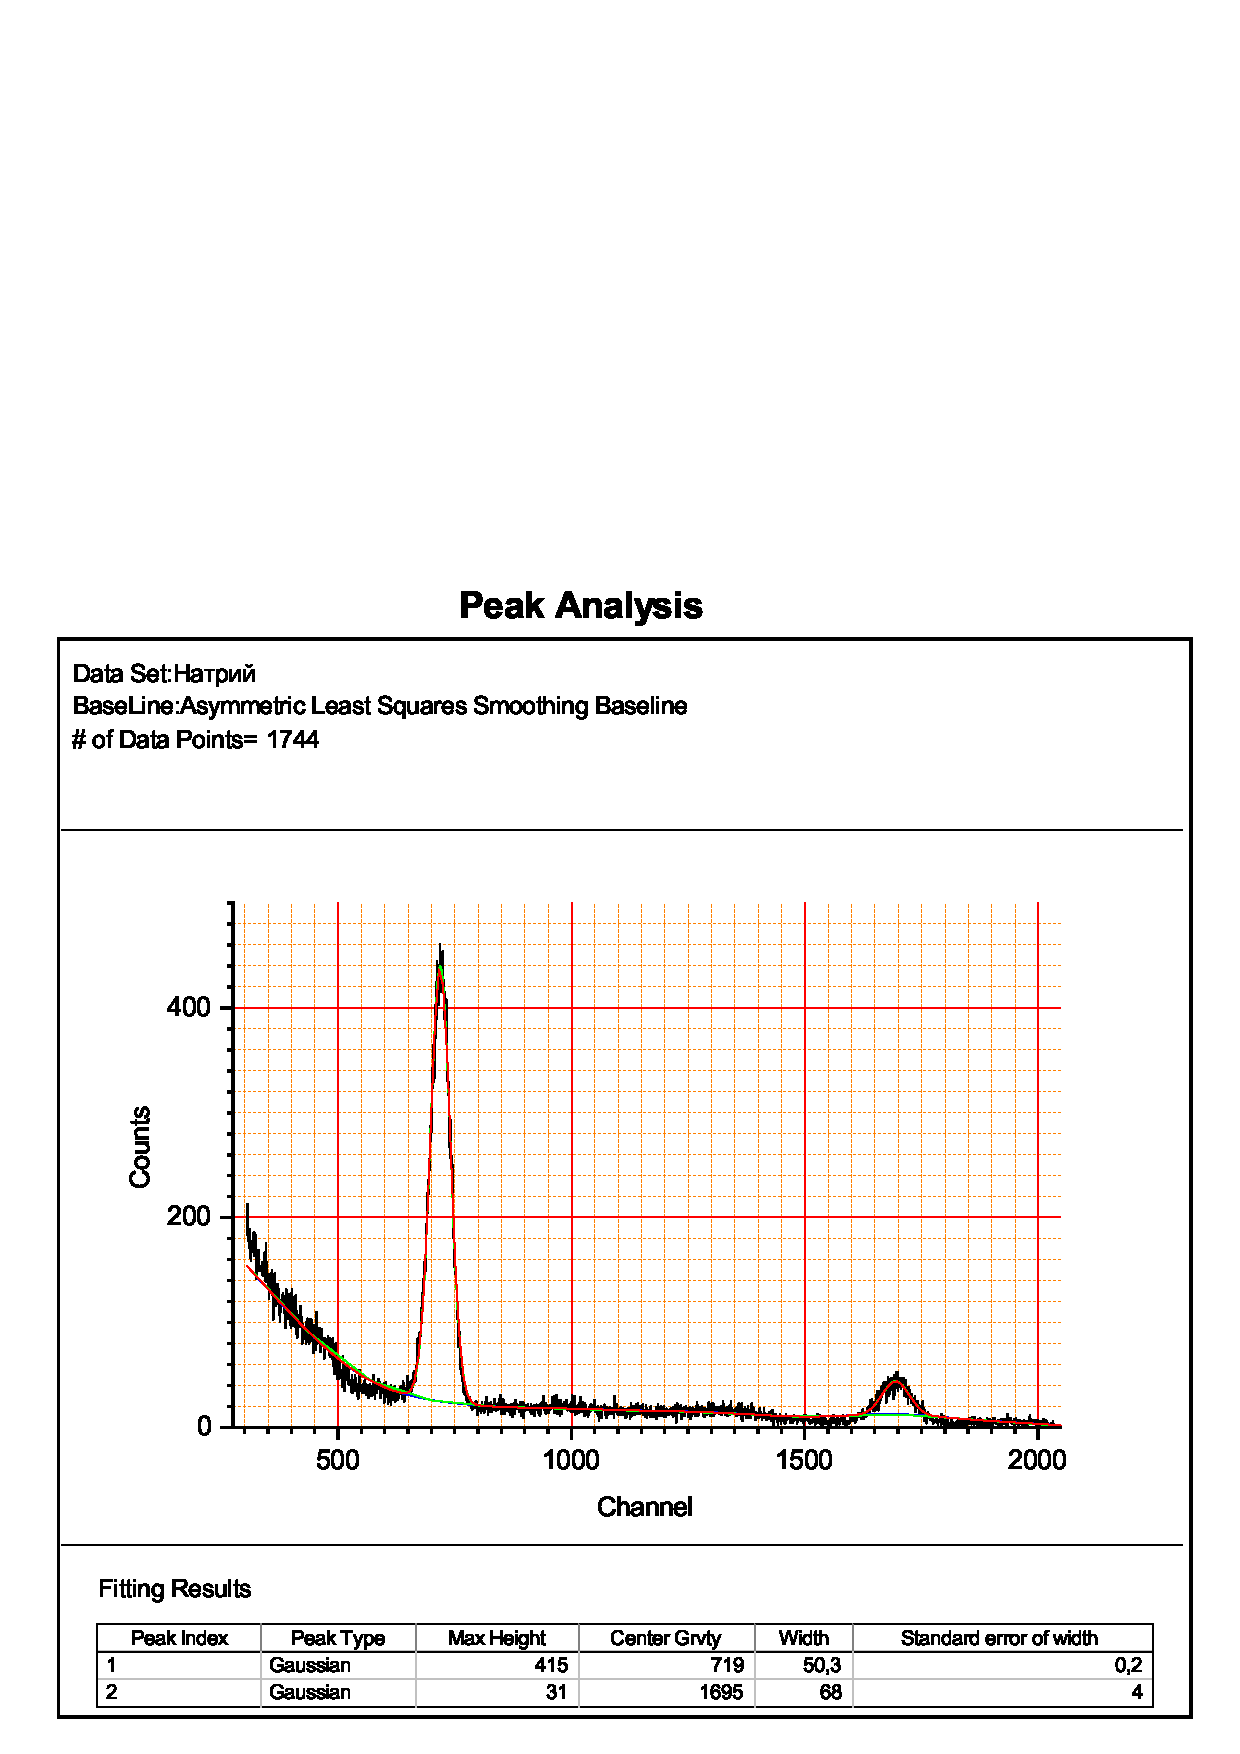
\includegraphics[width=0.7\linewidth]{1.jpg}\\
 
   \\
  
 \end{center}
 
 Откуда видно, что $\frac{V_1}{V_2} < 0.005$, a $\frac{a}{PV^2}<0.03$, ошибка метода измерений равна 4\%, тогда
 
 \begin{equation*}
PV=\nu RT
\end{equation*}
\begin{equation*}
L=\frac{ RT^2}{\mu P}\frac{dP}{dT} = - \frac{R}{\mu} \frac{d(lnP)}{d(\frac{1}{T})}
\end{equation*}

\section{Оборудование и инструментальные погрешности}

\textbf{В работе используются:} термостат; герметический сосуд, заполненный исследуемой жидкостью; отсчетный микроскоп.\\
\textbf{Инструментальные погрешности измерений:}\\
Градусник -- 0,2 K \\
Штангенциркуль -- 0,1 мм\\


\begin{center}
ЭКСПЕРИМЕНТАЛЬНАЯ УСТАНОВКА
\end{center}


\begin{center}
\begin{minipage}{0.47\textwidth}
  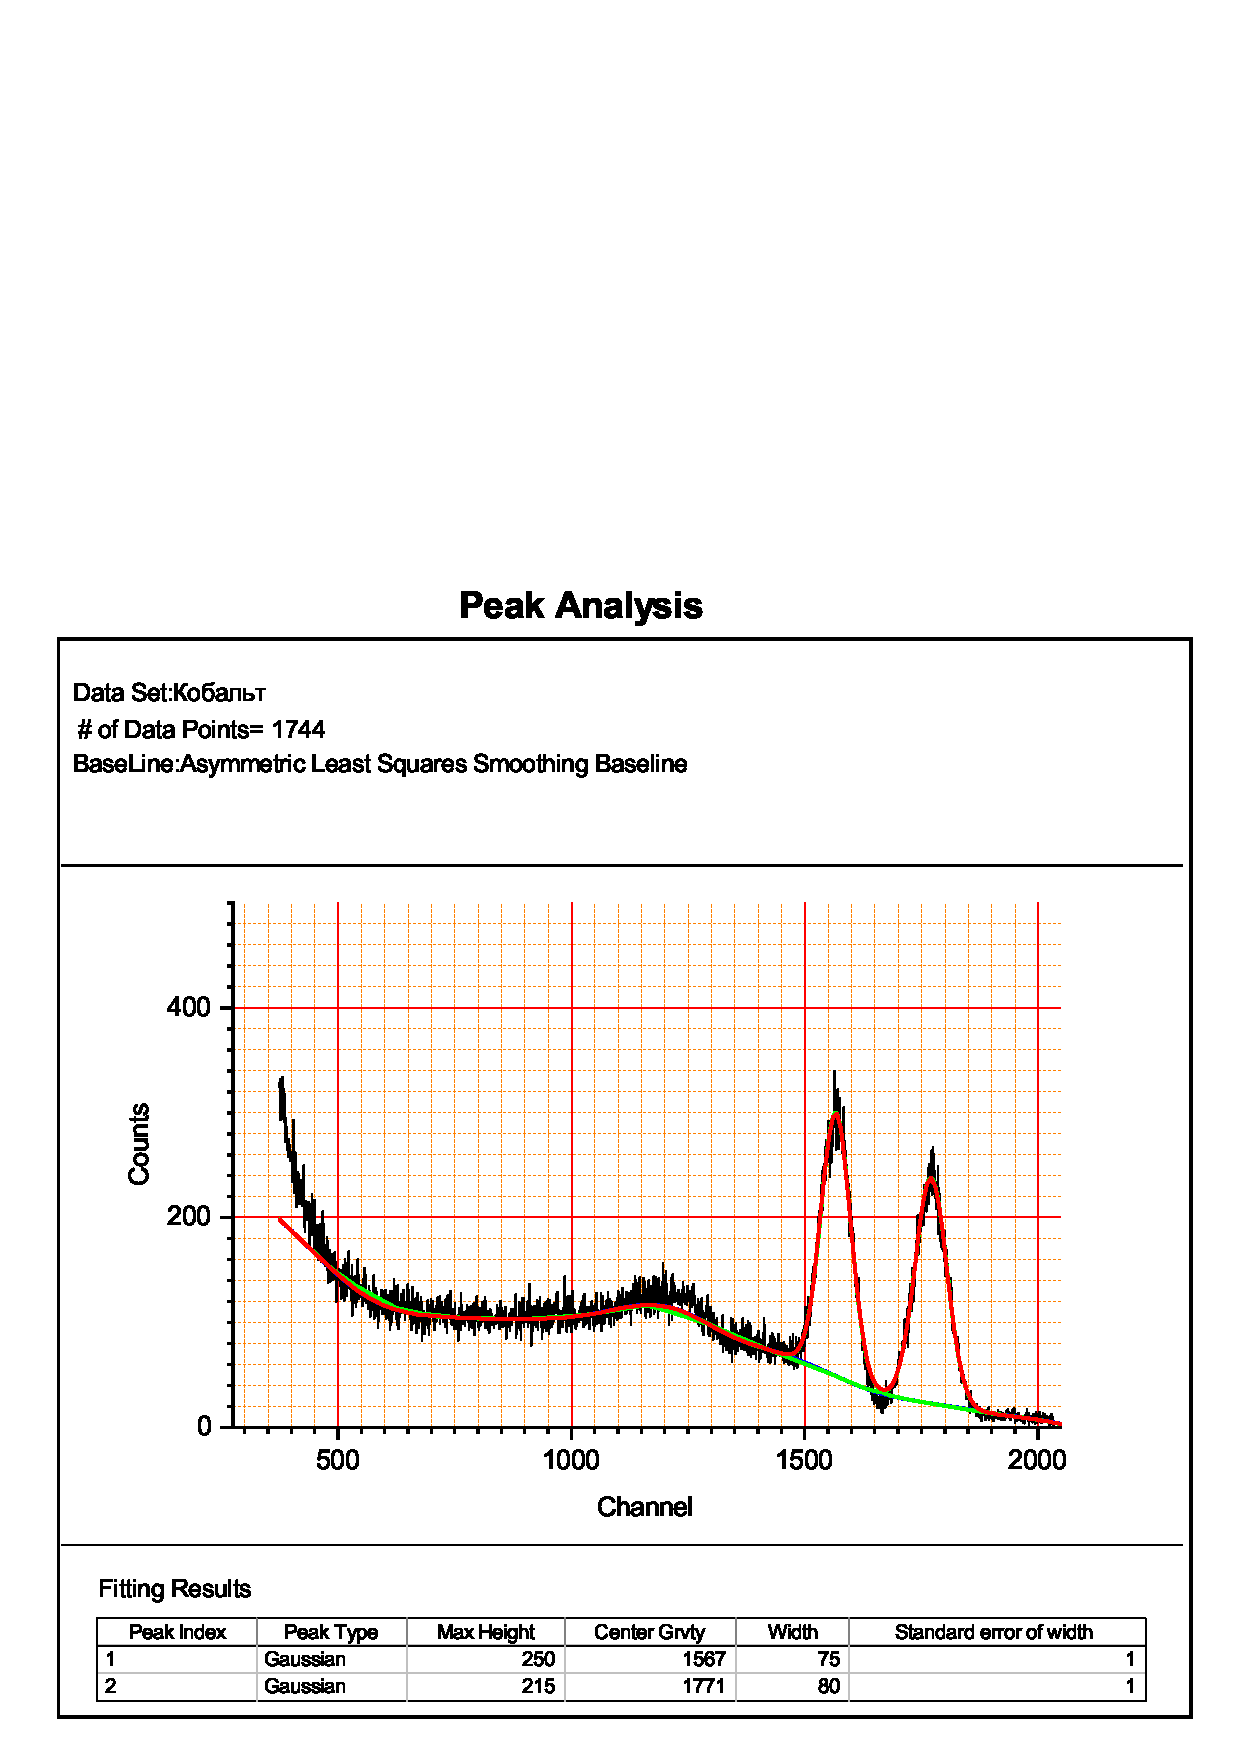
\includegraphics[width=1\linewidth]{2.jpg}
\end{minipage}
\begin{minipage}{0.04\textwidth}
\
\end{minipage}
\begin{minipage}{0.47\textwidth}
 На рисунке слева изображена схема установки.  Наполненный водой резервуар 1 играет роль термостата. Нагревание термостата производится спиралью 2, подогреваемой электрическим током. Для охлаждения воды в термостате через змеевик 3 пропускается водопроводная вода. Вода в термостате перемешивается воздухом, поступающим через трубку 4. Температура воды измеряется термометром 5. В термостат погружен запаянный прибор 6 с исследуемой жидкостью. Над ней находится насыщенный пар (перед заполнением прибора воздух из него был откачан). Давление насыщенного пара определяется по ртутному манометру, соединенному с исследуемым объемом. Отсчет показаний манометра производится при помощи микроскопа.\\
\end{minipage}
\end{center}

\section{Результаты измерений и обработка данных}

\subsection{Подготовка к эксперименту}
Измерим разность уровней в ртутном U - образном манометре с помощью микроскопа и температуру по термометру. Включим термостат. Через каждый градус будем измерять разность высот и температуру. Продолжим повышать температуру в течение половины имеющегося у нас времени, чтобы успеть произвести измерения при остывании прибора. Проведём те же измерения при охлаждении жидкости. Установим такой поток воды, чтобы охлаждение шло примерно тем же темпом, что и нагревание.
\\
\newpage
\subsection{Проведение измерений}\\

Измерим начальную разность уровней:

\begin{equation*}
	\Delta H _0 = 18.0 \pm 0.1 мм
\end{equation*}

Проведем измерения с шагом 1 градус при нагревании и последующем охлаждении системы. Результаты занесем в \textit{Таблицу 1}:

\begin{table}[h!]
\caption{Результаты измерений и их первичная обработка}
\begin{tabular}{|l|l|l|l|l|l|ll}
\hline
T, C                       & $H_{up}$, мм           & $H_{down}$, мм           & $\Delta H_{up}$, мм               & $\Delta H_{down}$, мм              & 1/T, 1/K $\cdot 10 ^ {-5}$ & \multicolumn{1}{l|}{$ln(\frac{P_{up}}{P_0})$} & \multicolumn{1}{l|}{$ln(\frac{P_{down}}{P_0})$} \\ \hline
20                         & 79.5                   & 79.6                     & 18.0                              & 17.8                               & 341.3                      & \multicolumn{1}{l|}{0.000}                    & \multicolumn{1}{l|}{-0.011}                     \\ \hline
21                         & 79.0                   & 79.1                     & 19.0                              & 18.8                               & 340.1                      & \multicolumn{1}{l|}{0.054}                    & \multicolumn{1}{l|}{0.043}                      \\ \hline
22                         & 78.7                   & 78.4                     & 19.6                              & 20.2                               & 339.0                      & \multicolumn{1}{l|}{0.085}                    & \multicolumn{1}{l|}{0.115}                      \\ \hline
23                         & 78.0                   & 78.0                     & 21.0                              & 21.0                               & 337.8                      & \multicolumn{1}{l|}{0.154}                    & \multicolumn{1}{l|}{0.154}                      \\ \hline
24                         & 77.4                   & 77.5                     & 22.2                              & 22.0                               & 336.7                      & \multicolumn{1}{l|}{0.210}                    & \multicolumn{1}{l|}{0.201}                      \\ \hline
25                         & 76.9                   & 77.0                     & 23.2                              & 23.0                               & 335.6                      & \multicolumn{1}{l|}{0.254}                    & \multicolumn{1}{l|}{0.245}                      \\ \hline
26                         & 76.2                   & 76.2                     & 24.6                              & 24.6                               & 334.4                      & \multicolumn{1}{l|}{0.312}                    & \multicolumn{1}{l|}{0.312}                      \\ \hline
27                         & 75.5                   & 75.4                     & 26.0                              & 26.2                               & 333.3                      & \multicolumn{1}{l|}{0.368}                    & \multicolumn{1}{l|}{0.375}                      \\ \hline
28                         & 74.8                   & 74.7                     & 27.4                              & 27.6                               & 332.2                      & \multicolumn{1}{l|}{0.420}                    & \multicolumn{1}{l|}{0.427}                      \\ \hline
29                         & 74.2                   & 73.8                     & 28.6                              & 29.4                               & 331.1                      & \multicolumn{1}{l|}{0.463}                    & \multicolumn{1}{l|}{0.491}                      \\ \hline
30                         & 73.5                   & 72.9                     & 30.0                              & 31.2                               & 330.0                      & \multicolumn{1}{l|}{0.511}                    & \multicolumn{1}{l|}{0.550}                      \\ \hline
31                         & 72.5                   & 72.2                     & 32.0                              & 32.6                               & 328.9                      & \multicolumn{1}{l|}{0.575}                    & \multicolumn{1}{l|}{0.594}                      \\ \hline
32                         & 71.7                   & 71.3                     & 33.6                              & 34.4                               & 327.9                      & \multicolumn{1}{l|}{0.624}                    & \multicolumn{1}{l|}{0.648}                      \\ \hline
33                         & 70.8                   & 70.0                     & 35.4                              & 37.0                               & 326.8                      & \multicolumn{1}{l|}{0.676}                    & \multicolumn{1}{l|}{0.721}                      \\ \hline
34                         & 69.7                   & 69.2                     & 37.6                              & 38.6                               & 325.7                      & \multicolumn{1}{l|}{0.737}                    & \multicolumn{1}{l|}{0.763}                      \\ \hline
35                         & 68.4                   & 68.0                     & 40.2                              & 41.0                               & 324.7                      & \multicolumn{1}{l|}{0.803}                    & \multicolumn{1}{l|}{0.823}                      \\ \hline
36                         & 67.6                   & 66.9                     & 41.8                              & 43.2                               & 323.6                      & \multicolumn{1}{l|}{0.843}                    & \multicolumn{1}{l|}{0.875}                      \\ \hline
37                         & 66.1                   & 65.9                     & 44.8                              & 45.2                               & 322.6                      & \multicolumn{1}{l|}{0.912}                    & \multicolumn{1}{l|}{0.921}                      \\ \hline
38                         & 65.0                   & 64.7                     & 47.0                              & 47.6                               & 321.5                      & \multicolumn{1}{l|}{0.960}                    & \multicolumn{1}{l|}{0.972}                      \\ \hline
39                         & 63.8                   & 63.7                     & 49.4                              & 49.6                               & 320.5                      & \multicolumn{1}{l|}{1.010}                    & \multicolumn{1}{l|}{1.014}                      \\ \hline
40                         & 62.4                   & 62.4                     & 52.2                              & 52.2                               & 319.5                      & \multicolumn{1}{l|}{1.065}                    & \multicolumn{1}{l|}{1.065}                      \\ \hline
$\sigma T$ $\approx$ 0.2 & \multicolumn{2}{l|}{$\sigma H$ $\approx$ 0.1} & \multicolumn{2}{l|}{$\sigma \Delta H$ = 2 $\sigma H$ $\approx$ 0.2} & $\sigma 1/T$ $\approx$ 0.3 & \multicolumn{2}{l}{}                                                                            \\ \cline{1-6}
\end{tabular}
\end{table}
\subsection{Обработка результатов измерений}

В нее же занесем погрешности и результаты обработки измерений:

\begin{equation*}
\Delta H = \Delta H_0 - 2 H + 2 H_0
\end{equation*}
\:\:\:\:\:\:\:\:\:\:\:\:\:\:\:\:\:\:\:\:\:\:\:\:\:\:\:\:\:\:\:\:\:\:\:\:\:\:\:\:\:\:\:\:\:\:\:\:\:\:\:\:\:, где $H_0$ - высота при температуре 20 С
\begin{equation*}
ln(\frac{P}{P_0}) = ln(\frac{\Delta H}{\Delta H_0})
\end{equation*}

\begin{equation*}
\sigma ln(\frac{P}{P_0}) \approx \frac{2\sigma \Delta H}{\Delta H} \approx 0.015
\end{equation*}

Сначала построим график зависимости $\Delta H$ от $T$ (по сути $\Delta P$ от $T$). На одни оси нанесем данные повышения и понижения температуры. Построим ту же зависимость в координатах $1/T$ от $ln(\frac{P}{P_0})$ на другом графике:

\begin{tikzpicture}[scale=1.7]
	\begin{axis}[
		grid = both,
		grid style={line width=.1pt, draw=gray!10},
    major grid style={line width=.2pt,draw=gray!50},
    minor tick num=5,
    enlargelimits={abs=0.5},
		axis lines = left,
    	xlabel = {T, C},
    	ylabel = {$\Delta H$, мм},
    	ylabel style={black, scale=0.7},
    	xlabel style={black, scale=0.7},
    	xmin=15, xmax=45
		]
		\addplot +[blue, only marks,
		] plot[
			error bars/.cd,
			y dir=both,
			y fixed=0,
			x dir=both,
			x fixed=0,
		] table [		    	    	    	
			x=T, 
			y=dH1,
		]{DataGr.csv};

		\addplot +[red, only marks,
		] plot[
			error bars/.cd,
			y dir=both,
			y fixed=0,
			x dir=both,
			x fixed=0,
		] table [		    	    	    	
			x=T, 
			y=dH2,
		]{DataGr.csv};
	

	\end{axis}
\end{tikzpicture}

\begin{tikzpicture}[scale=1.7]
	\begin{axis}[
		grid=both,
    grid style={line width=.1pt, draw=gray!10},
    major grid style={line width=.2pt,draw=gray!50},
    minor tick num=5,
    enlargelimits={abs=0.5},
		axis lines = left,
    	xlabel = {1/T, 1/k $\cdot 10^{-4}$},
    	ylabel = {$ln(\frac{P}{P_0})$},
    	ylabel style={black, scale=0.7},
    	xlabel style={black, scale=0.7},
    	xmin=319, xmax=345
		]
		\addplot +[blue, only marks,
		] plot[
			error bars/.cd,
			y dir=both,
			y fixed=0,
			x dir=both,
			x fixed=0,
		] table [		    	    	    	
			x=TT, 
			y=P1,
		]{DataGr.csv};

		\addplot +[red, only marks,
		] plot[
			error bars/.cd,
			y dir=both,
			y fixed=0,
			x dir=both,
			x fixed=0,
		] table [		    	    	    	
			x=TT, 
			y=P2,
		]{DataGr.csv};
		\addplot[color=green, domain=319:345]{16.746915 - 0.049133 * x};
	

	\end{axis}
\end{tikzpicture}

Заметно небольшое различие зависимостей давления от температуры при нагревании и охлаждении. \\

\newpage

\textbf{$\Delta H$ от $T$:} Для нахождения L необходимо сосчитать производную в каждой точке, для этого воспользуемся методом сплайнов "в первом приближении" (так же будем учитывать строгую монотонность производной в силу итак большой погрешности эксперимента), для чего по каждым трём точкам мысленно построим параболу и найдем её угловой коэффициент для зависимти $\Delta H$ от $T$. Полученные результаты занесем в \textit{Таблицу 2}. Далее найдём среднее значение теплоты испарения. \\

\begin{table}[h!]
\centering
\caption{Вычисление касательных к графику}
\begin{tabular}{|l|l|l|l|l|}
\hline
T  & $\frac{dP}{dT}_{up}$, Па/К & $\frac{dP}{dT}_{down}$, Па/К & $L_{up}$, кДж/кг & $L_{down}$, кДж/кг \\ \hline
21 & 7.84                       & 11.76                        & 1678             & 2545               \\ \hline
22 & 9.80                       & 10.78                        & 2048             & 2186               \\ \hline
23 & 12.74                      & 8.82                         & 2501             & 1732               \\ \hline
24 & 10.78                      & 9.80                         & 2016             & 1849               \\ \hline
25 & 11.76                      & 12.74                        & 2118             & 2315               \\ \hline
26 & 13.72                      & 15.68                        & 2347             & 2682               \\ \hline
27 & 13.72                      & 14.70                        & 2235             & 2376               \\ \hline
28 & 12.74                      & 15.68                        & 1982             & 2422               \\ \hline
29 & 12.74                      & 17.64                        & 1912             & 2575               \\ \hline
30 & 16.66                      & 15.68                        & 2399             & 2171               \\ \hline
31 & 17.64                      & 15.68                        & 2397             & 2092               \\ \hline
32 & 16.66                      & 21.56                        & 2171             & 2744               \\ \hline
33 & 19.60                      & 20.58                        & 2440             & 2451               \\ \hline
34 & 23.52                      & 19.60                        & 2775             & 2252               \\ \hline
35 & 20.58                      & 22.54                        & 2285             & 2454               \\ \hline
36 & 22.54                      & 20.58                        & 2423             & 2141               \\ \hline
37 & 25.48                      & 21.56                        & 2572             & 2157               \\ \hline
38 & 22.54                      & 21.56                        & 2183             & 2062               \\ \hline
39 & 25.48                      & 22.54                        & 2363             & 2082               \\ \hline
\multicolumn{5}{|l|}{$L_{ср}$ = $(2.3 \pm 0.3) \cdot 10 ^{6}$ Дж/кг}                                  \\ \hline
\end{tabular}
\end{table}

К статистической погрешности прбавим приборную погрешность и получим:

\begin{equation*}
L = 2.3 \pm 0.3  \: МДж/кг
\end{equation*}

\\

\textbf{$ln(\frac{P}{P_0})$ от $1/T$:} График и так линеен, поэтому найдем его угловой коэффициент и напрямую из него L:

\begin{equation*}
L = 2.27 \pm 0.04 \: МДж/кг
\end{equation*}

Полезно будет сравнить результаты с табличными значениями:

\begin{equation*}
L_{табл} = 2.26 \: МДж/кг
\end{equation*}







\newpage

 \section{Выводы}
 
Оба метода дают результаты совпадающие с табличными значениями. Что также подтверждает, что наша оценка применимости модели, которую мы провели в начале работы, была верна.

Точности двух методов вычисления значительно отличаются; вероятно из-за большого влияния погрешности измерений на точечные вычисления производной. График в осях $ln(P)$ от $1/T$ более информативен и нагляден и является предпочтительным при вычислении L.

Разница данных при нагревании и при охлаждении ,в основном, лежит в пределах погрешности измерений и никаких тенденций в отклонениях не наблюдается. \\


\end{document}
